\documentclass[12pt,landscape]{article}
\usepackage[english,greek]{babel}
\usepackage[utf8]{inputenc}
\usepackage{xparse}
\usepackage{nimbusserif}
\usepackage[T1]{fontenc}
\usepackage[left=2.00cm, right=2.00cm, top=3.00cm, bottom=2.00cm,a2paper]{geometry}
\usepackage{multicol,longtable,multirow,hhline,enumitem,tikz,pgfplots,tkz-euclide,tkz-tab,capt-of,fontawesome5,gensymb,tabularray,fancyhdr,etoolbox,eurosym,xcolor-material,siunitx,eqparbox,lipsum}
\usetikzlibrary{arrows.meta}
\usepackage[most]{tcolorbox}
\usetikzlibrary{tikzmark}
\let\myBbbk\Bbbk
\let\Bbbk\relax
\usepackage[curlybraces,amsbb,mtphrb]{mtpro2}
\usepackage[explicit]{titlesec}
\usepackage{soul}
\newcommand{\eng}{\selectlanguage{english}}
\newcommand{\gr}{\selectlanguage{greek}}
\usepackage{mathimatika}
%\usepackage[usenames,dvipsnames,cmyk,table,x11names]{xcolor}
\def\xrwma{red!80!black}
\definecolor{steelblue}{cmyk}{.7,.278,0,.294}
\definecolor{doc}{cmyk}{1,0.455,0,0.569}
\definecolor{orange}{HTML}{ff7300}

\newcommand{\ekthetesdeiktes}{\DeclareMathSizes{10.95}{10.95}{7}{5}
\DeclareMathSizes{6}{6}{3.8}{2.7}
\DeclareMathSizes{8}{8}{5.1}{3.6}
\DeclareMathSizes{9}{9}{5.8}{4.1}
\DeclareMathSizes{10}{10}{6.4}{4.5}
\DeclareMathSizes{12}{12}{7.7}{5.5}
\DeclareMathSizes{14.4}{14.4}{9.2}{6.5}
\DeclareMathSizes{17.28}{17.28}{11}{7.9}
\DeclareMathSizes{20.74}{20.74}{13.3}{9.4}
\DeclareMathSizes{24.88}{24.88}{16}{11.3}

\makeatletter
\newcommand{\subsup}{
\AtBeginDocument{
\check@mathfonts
\fontdimen16\textfont2=2.5pt
\fontdimen17\textfont2=2.5pt
\fontdimen14\textfont2=4.5pt
\fontdimen13\textfont2=4.5pt}
}
\makeatother}
\usepackage{wrapfig}
\newenvironment{WrapText1}[3][r]
{\wrapfigure[#2]{#1}{#3}}
{\endwrapfigure}

\newenvironment{WrapText2}[3][l]
{\wrapfigure[#2]{#1}{#3}}
{\endwrapfigure}
\newcommand{\wrapr}[6]{
\begin{minipage}{\linewidth}\mbox{}\\
\vspace{#1}
\begin{WrapText1}{#2}{#3}
\vspace{#4}#5\end{WrapText1}#6
\end{minipage}}

\newcommand{\wrapl}[6]{
\begin{minipage}{\linewidth}\mbox{}\\
\vspace{#1}
\begin{WrapText2}{#2}{#3}
\vspace{#4}#5\end{WrapText2}#6
\end{minipage}}
\usepackage{etoolbox,hhline,moreenum}
\usepackage{caption} 
\captionsetup[table]{skip=5pt}
\makeatletter
\newif\ifLT@nocaption
\preto\longtable{\LT@nocaptiontrue}
\appto\endlongtable{%
\ifLT@nocaption
\addtocounter{table}{\m@ne}%
\fi}
\preto\LT@caption{%
\noalign{\global\LT@nocaptionfalse}}
\makeatother

\newlist{alist}{enumerate}{1}
\setlist[alist]{label=\let\textdexiakeraia\relax\alph*.}
\UseTblrLibrary{counter}

\pgfmathdeclarefunction{gauss}{2}{%
\pgfmathparse{1/(#2*sqrt(2*pi))*exp(-((x-#1)^2)/(2*#2^2))}%
}
\pgfkeys{/pgfplots/aks_on/.style={axis lines=center,
xlabel style={at={(current axis.right of origin)},xshift=1.5ex,anchor=center},
ylabel style={at={(current axis.above origin)},yshift=1.5ex, anchor=center}}}
\pgfkeys{/pgfplots/grafikh parastash/.style={red!80!black,line width=.4mm,samples=200}}
\pgfkeys{/pgfplots/belh ar/.style={tick label style={font=\scriptsize},axis line style={-latex}}}
\tikzstyle{pl}=[line width=0.3mm]
\tikzstyle{plm}=[line width=0.4mm]

\newcommand{\kerkissans}[1]{{\fontfamily{maksf}\selectfont {#1}}}
\AtBeginDocument{\renewcommand{\textstigma}{\textsigma\texttau}}

\definecolor{titlecolor}{HTML}{cd0f00}

\newbox\TitleUnderlineTestBox
\newcommand*\TitleUnderline[1]
{%
\bgroup
\setbox\TitleUnderlineTestBox\hbox{\colorbox{titleblue}\strut}%
\setul{\dimexpr\dp\TitleUnderlineTestBox-.3ex\relax}{.3ex}%
\ul{#1}%
\egroup
}
\newcommand*\SectionNumberBox[1]
{%
\colorbox{red!80!black}
{%
\makebox[2em][c]
{%
\color{white}%
\strut
\csname the#1\endcsname
}%
}%
\TitleUnderline{\ \ \ }%
}

\titleformat{\section}[hang]
{\Large\fontfamily{maksf}\selectfont}%
{\colorbox{\xrwma}{%
\raisebox{0pt}[13pt][3pt]{\makebox[80pt]{% height, width
\color{white}{\kerkissans{\textbf{\thesection ο Κεφάλαιο}}}}%
}}}%
{0pt}%
{\colorbox{black}{\raisebox{0pt}[13pt][3pt]{\color{white}\ \textbf{#1}\ }}}

\titleformat{\subsection}[hang]
{\large\bfseries\fontfamily{maksf}\selectfont}%
{\colorbox{red!80!black}{%
\raisebox{0pt}[13pt][3pt]{\makebox[30pt]{% height, width
\color{white}{\kerkissans{\textbf{\thesubsection}}}}%
}}}%
{0pt}%
{\colorbox{black}{\raisebox{0pt}[13pt][3pt]{\color{white}\ \textbf{#1}\ }}}

\makeatletter
\@addtoreset{section}{part}
\makeatother

\titleformat{\part}[display]
{\normalfont\huge\filcenter\bfseries}{}{-30pt}{\Huge \textcolor{red!80!black}{ \kerkissans{ #1}}}
\titlespacing*{\part} 
{0pt}{0pt}{0pt}

\setlist[enumerate]{itemsep=0mm,label=\textcolor{\xrwma}{\textbf{\arabic*.}}}
\definecolor{bblue}{HTML}{4F81BD}
\definecolor{rred}{HTML}{C0504D}
\definecolor{ggreen}{HTML}{9BBB59}
\definecolor{ppurple}{HTML}{9F4C7C}

\makeatletter
\usetikzlibrary{patterns}
\tikzstyle{chart}=[
legend label/.style={font={\scriptsize},anchor=west,align=left},
legend box/.style={rectangle, draw, minimum size=5pt},
axis/.style={black,semithick,->},
axis label/.style={anchor=east,font={\tiny}},
]

\tikzstyle{bar chart}=[
chart,
bar width/.code={
\pgfmathparse{##1/2}
\global\let\bar@w\pgfmathresult
},
bar/.style={very thick, draw=white},
bar label/.style={font={\bf\small},anchor=north},
bar value/.style={font={\footnotesize}},
bar width=.75,
]

\tikzstyle{pie chart}=[
chart,
slice/.style={line cap=round, line join=round,thick,draw=white},
pie title/.style={font={\bf}},
slice type/.style 2 args={
##1/.style={fill=##2},
values of ##1/.style={}
}
]

\pgfdeclarelayer{background}
\pgfdeclarelayer{foreground}
\pgfsetlayers{background,main,foreground}

\newcommand{\pie}[3][]{
\begin{scope}[#1]
\pgfmathsetmacro{\curA}{90}
\pgfmathsetmacro{\r}{1}
\def\c{(0,0)}
\node[pie title] at (90:1.3) {#2};
\foreach \v/\s/\l in{#3}{
\pgfmathsetmacro{\deltaA}{\v/100*360}
\pgfmathsetmacro{\nextA}{\curA + \deltaA}
\pgfmathsetmacro{\midA}{(\curA+\nextA)/2}

\path[slice,\s] \c
-- +(\curA:\r)
arc (\curA:\nextA:\r)
-- cycle;
\pgfmathsetmacro{\d}{max((\deltaA * -(.5/50) + 1) , .5)}

\begin{pgfonlayer}{foreground}
\path \c -- node[pos=\d,pie values,values of \s]{$\l$} +(\midA:\r);
\end{pgfonlayer}

\global\let\curA\nextA
}
\end{scope}
}

\newcommand{\legend}[2][]{
\begin{scope}[#1]
\path
\foreach \n/\s in {#2}
{
++(0,-10pt) node[\s,legend box] {} +(5pt,0) node[legend label] {\n}
}
;
\end{scope}
}
\definecolor{a}{cmyk}{0,1,1,0.05}
\definecolor{b}{cmyk}{0,.8,.8,.15}
\definecolor{c}{cmyk}{0,.8,.8,.0}
\definecolor{d}{cmyk}{0,.7,.7,0}
\definecolor{e}{cmyk}{0,.5,.5,0}

\pgfplotsset{every axis/.append style={
x tick label style={/pgf/number format/.cd, 1000 sep={.}}}}

\fancyhf{}
\newcommand{\myleftmark}{\leftmark}
\renewcommand{\myleftmark}{{\Large Τυπολόγιο}}
\renewcommand{\headrulewidth}{0pt}
\renewcommand{\sectionmark}[1]{\markboth{\large Κεφάλαιο \thesection\ -\ #1}{} }


%-------- ΠΑΡΑΤΗΡΗΣΕΙΣ -----------------
\newcounter{parathrhsh}[section]
\renewcommand{\theparathrhsh}{\arabic{parathrhsh}}  
\newcommand{\Parathrhsh}[1]{\refstepcounter{parathrhsh}{\textbf{\textcolor{white}{\faLightbulb}\ \ -\ \ \kerkissans{Παρατήρηση\hspace{2mm}\theparathrhsh}}}}{}

\newcommand{\tss}[1]{\textsuperscript{#1}}
\newcommand{\tssL}[1]{\MakeLowercase{\textsuperscript{#1}}}

%----------- ΠΑΡΑΤΗΡΗΣΗ------------------
\newenvironment{parat}[1]
{\begin{tcolorbox}[toptitle=1mm,
bottomtitle=1mm,title=\Parathrhsh,
breakable,
enhanced standard,lifted shadow={1mm}{-2mm}{3mm}{0.3mm}%
{black!50!white},
colback=red!5!white,
boxrule=0.1pt,
colframe=red!80!black,
fonttitle=\bfseries,width=#1]}
{\end{tcolorbox}}
%-----------------------------------------

%----------- ΑΣΚΗΣΗ ------------------
\newcounter{askhsh}[section]
\renewcommand{\theaskhsh}{\thesection.\arabic{askhsh}}   
\newcommand{\Askhsh}{\refstepcounter{askhsh}{\textbf{\textcolor{\xrwma}{\faPenSquare\ \  \large \kerkissans{\textbf{Άσκηση\hspace{2mm}\theaskhsh}}}}}\hspace{1mm}}{}
%------------------------------------
\newenvironment{askhsh}[1]
{\begin{tcolorbox}[title=\Askhsh\ \ :\ \  {\textcolor{black}{\kerkissans{\bmath{#1}}}},breakable,
enhanced standard,titlerule=-.2pt,toprule=0pt, rightrule=0pt, bottomrule=0pt,
colback=white,left=2mm,top=1mm,bottom=0mm,
boxrule=0pt,
colframe=white,borderline west={1.5mm}{0pt}{\xrwma},leftrule=2mm,sharp corners,coltitle=\xrwma]}
{\end{tcolorbox}}
%-----------------------------------------

%------- ΣΤΥΛ ΠΑΡΑΔΕΙΓΜΑΤΟΣ -------
\newcounter{paradeigma}[section]
\renewcommand{\theparadeigma}{\kerkissans{\arabic{paradeigma}}}   
\newcommand{\Paradeigma}[1]{\refstepcounter{paradeigma}\kerkissans{\bmath{\textcolor{red!80!black}{\faPlay\large \ \ Παράδειγμα\hspace{2mm}\theparadeigma\;:\;}\hspace{1mm}  #1}}\\}{}
%-----------------------------------

%------- ΣΤΥΛ ΛΥΣΗΣ ------------------
\newcommand{\lysh}{\textcolor{\xrwma}{\kerkissans{\noindent\faCheck\ \textbf{ΛΥΣΗ}}}\\}
%------------------------------------

%-------- ΠΡΟΣΟΧΗ -----------------
\newcounter{prosoxi}[section]
\renewcommand{\theprosoxi}{\arabic{prosoxi}}  
\newcommand{\Prosoxi}[1]{\refstepcounter{prosoxi}{\faExclamationTriangle\ \ \ \textbf{Προσοχή\hspace{2mm}\thesection.\theprosoxi}}}{}

%----------- ΠΡΟΣΟΧΗ------------------
\newenvironment{prosoxi}[1]
{\begin{tcolorbox}[title=\Prosoxi,
breakable,
enhanced standard,lifted shadow={1mm}{-2mm}{3mm}{0.3mm}%
{black!50!white},
colback=red!5!white,
boxrule=0.1pt,
colframe=red!80!black,
fonttitle=\bfseries,width=#1]}
{\end{tcolorbox}}
%-----------------------------------------

\DeclareTblrTemplate{caption}{nocaptemplate}{}
\DeclareTblrTemplate{capcont}{nocaptemplate}{}
\DeclareTblrTemplate{contfoot}{nocaptemplate}{}
\NewTblrTheme{mytabletheme}{
  \SetTblrTemplate{caption}{nocaptemplate}{}
  \SetTblrTemplate{capcont}{nocaptemplate}{}
  \SetTblrTemplate{contfoot}{nocaptemplate}{}
}

\NewTblrEnviron{mytblr}
\SetTblrStyle{firsthead}{font=\bfseries}
\SetTblrStyle{firstfoot}{fg=red2}
\SetTblrOuter[mytblr]{theme=mytabletheme}
\SetTblrInner[mytblr]{
rowspec={t{7mm}},columns = {c},
  width = 0.85\linewidth,
  row{odd} = {bg=red9,fg=black,ht=8mm},
 row{even} = {bg=red7,fg=black,ht=8mm},
hlines={white},vlines={white},
row{1} = {bg=red4, fg=white, font=\bfseries\fontfamily{maksf}},rowhead = 1,
  hline{2} = {.7mm}, % midrule  
}


\DeclareRobustCommand{\officialeuro}{%
  \ifmmode\expandafter\text\fi
  {\fontencoding{U}\fontfamily{eurosym}\selectfont e}}

\titleformat{\paragraph}
{\normalfont\huge }%
{}{0em}%
{{\color{black}\titlerule[0pt]}\vskip-.2\baselineskip{\parbox[t]{\dimexpr\textwidth-2\fboxsep\relax}{\raggedright\strut{{\textcolor{red!80!black}{\faSquare\ \ \kerkissans{\bmath{#1}}}}}\strut}}}[\vskip -.2\baselineskip{}]
\setlength{\parindent}{0pt}

\begin{document}
\begin{multicols}{3}
\paragraph{Τριγωνομετρικοί αριθμοί}
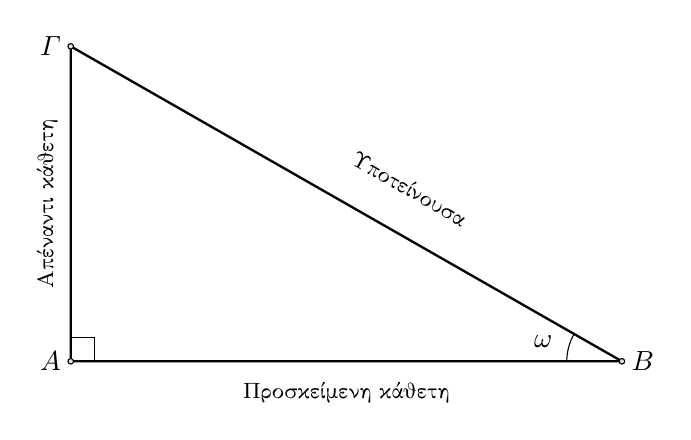
\begin{tikzpicture}
\tkzDefPoint(0,0){A}
\tkzDefPoint(7,0){B}
\tkzDefPoint(0,4){C}
\tkzMarkAngle[fill=red7,size=.7](C,B,A)
\tkzMarkRightAngle[size=.3](B,A,C)
\tkzDrawPolygon[pl](A,B,C)
\tkzText(6,.25){$ \omega $}
\tkzLabelPoint[left](A){$ A $}
\tkzLabelPoint[right](B){$ B $}
\tkzLabelPoint[left](C){$ \varGamma $}
\tkzDrawPoints(A,B,C)
\node[rotate=-29.74] at(4.3,2.2){{\footnotesize Υποτείνουσα}};
\node[rotate=90] at(-.3,2){{\footnotesize Απέναντι κάθετη}};
\node at(3.5,-.4){{\footnotesize Προσκείμενη κάθετη}};
\end{tikzpicture}
\begin{itemize}
\item $\textrm{Ημίτονο}=\dfrac{\textrm{Απέναντι Κάθετη}}{\textrm{Υποτείνουσα}}\;\;,\;\;\hm{\omega}=\dfrac{A\varGamma}{B\varGamma}$
\item $\textrm{Συνημίτονο}=\dfrac{\textrm{Προσκείμενη Κάθετη}}{\textrm{Υποτείνουσα}}\;\;,\;\;\syn{\omega}=\dfrac{AB}{B\varGamma} $
\item $\textrm{Εφαπτομένη}=\dfrac{\textrm{Απέναντι Κάθετη}}{\textrm{Προσκείμενη Κάθετη}}\;\;,\;\;\ef{\omega}=\dfrac{A\varGamma}{AB}$
\item $\textrm{Συνεφαπτομένη}=\dfrac{\textrm{Προσκείμενη Κάθετη}}{\textrm{Απέναντι Κάθετη}}\;\;,\;\;\syf{\omega}=\dfrac{AB}{A\varGamma}$
\end{itemize}
\begin{tikzpicture}[y=.8cm,x=.9cm,scale=2]
\draw[draw=black,fill=\xrwma!50] (0,0) -- (.5,0) arc (0:40:.5) -- cycle;
\draw[-latex]  (-.4,0)  -- coordinate (x axis mid) (4,0) node[right,fill=white] {{ $ x $}};
\draw[-latex] (0,-.4) -- (0,3.5) node[above,fill=white] {{ $ y $}};
\draw (3,.1) -- (3,-.1) node[anchor=north] { $ x $};
\draw (.1,2.5) -- (-.1,2.5) node[anchor=east] { $ y $};
\draw[dashed] (3,0) -- (3,2.5) -- (0,2.5);
\tkzDefPoint(0,0){O}
\tkzDefPoint(3,2.5){M}
\tkzDefPoint(3,0){A}
\tkzDefPoint(0,2.5){B}
\tkzDrawSegment(O,M)
\tkzDrawPoints[fill=white](M,A,B)
\tkzLabelPoint[below left](O){$ O $}
\tkzLabelPoint[above](M){{ $ M(x,y) $}}
\tkzLabelPoint[above right](A){{ $ A(x,0) $}}
\tkzLabelPoint[above right](B){{ $ B(0,y) $}}
\tkzText(1.5,-.4){$ \undercbrace{\rule{43mm}{0mm}}_{{ x}} $}
\tkzText(-.3,1.25){{{ $ y $}}$\LEFTRIGHT\{.{ \rule{0pt}{40mm} } $}
\tkzText[fill=white,inner sep=.2mm](2.7,1){{ $ \rho=\sqrt{x^2+y^2} $}}
\tkzText(.7,.2){{ $ \omega $}}
\end{tikzpicture}
\[ \hm{\omega}=\frac{AM}{OM}=\frac{y}{\rho} \]

\textbf{Συνημίτονο}\\
Συνημίτονο της γωνίας $ \omega $ ονομάζεται ο λόγος της τετμημένης του σημείου προς την απόσταση του από την αρχή των αξόνων.
\[ \syn{\omega}=\frac{BM}{OM}=\frac{x}{\rho} \]
 \textbf{Εφαπτομένη}\\
Εφαπτομένη της γωνίας $ \omega $ ονομάζεται ο λόγος της τεταγμένης του σημείου προς την τετμημένη του.
\[ \ef{\omega}=\frac{AM}{BM}=\frac{y}{x}\;\;,\;\;x\neq0 \]
 \textbf{Συνεφαπτομένη}\\
Συνεφαπτομένη της γωνίας $ \omega $ ονομάζεται ο λόγος της τετμημένης του σημείου προς την τεταγμένη του.
\[ \syf{\omega}=\frac{BM}{AM}=\frac{x}{y}\;\;.\;\;y\neq0 \]
\usetikzlibrary{calc}
\tikzset{curveinscope/.style={every path/.style={draw=black, text=black}}}
\paragraph{Τριγωνομετρικός κύκλος}
\begin{center}
\begin{tikzpicture}[curveinscope,scale=0.95]
\draw[line width=.7mm] (0,0) circle(7);
\foreach \s in {0,1,2,...,359}{
\draw (\s:6.7)--(\s:7);
}

\foreach \s in {0,1,2,...,627}{
\draw (\s/628*360:7.3)--(\s/628*360:7);
}
\foreach \s in {0,5,10,...,625}{
\draw (\s/628*360:7.5)--(\s/628*360:7);
}
\foreach \s in {0,10,20,...,620}{
\draw (\s/628*360:7.7)--(\s/628*360:7);
\node at (\s/628*360:8){\pgfmathparse{0.01*\s}% Evaluate the expression
\pgfmathprintnumber[    % Print the result
fixed,
fixed zerofill,
precision=1
]{\pgfmathresult}};
}
\foreach \gwnia/\xtext in {
30/\dfrac{\pi}{6},
45/\dfrac{\pi}{4},
60/\dfrac{\pi}{3},
90/\dfrac{\pi}{2},
120/\dfrac{2\pi}{3},
135/\dfrac{3\pi}{4},
150/\dfrac{5\pi}{6},
180/\pi,
210/\dfrac{7\pi}{6},
225/\dfrac{5\pi}{4},
240/\dfrac{4\pi}{3},
270/\dfrac{3\pi}{2},
300/\dfrac{5\pi}{3},
315/\dfrac{7\pi}{4},
330/\dfrac{11\pi}{6},
360/2\pi}
{\draw (\gwnia:9.2) node {\textcolor{red4}{ $\xtext$}};
\draw(\gwnia:8.7)--(\gwnia:8.3);}
\draw[pl,-latex,black] (5,0.5) arc (5.7106:40:5.0249);
\draw[pl,-latex,black] (5,-0.5) arc (-5.7106:-40:5.0249);
\foreach \d in {0,10,20,...,350}{
\draw[pl] (\d:7)--(\d:6.4);
\node at (\d:5.9){\large$\d\degree$};
}
\foreach \d in {0,5,10,...,355}{
\draw[pl] (\d:7)--(\d:6.6);
}
\node at (4,2) {$+$};
\node at (4,-2) {$-$};
\foreach \d in {-0.8,-0.6,-0.4,-0.2,0.2,0.4,0.6,0.8}{
\draw (\d*5,-.1)node[yshift=-3mm]{$\d$}--(\d*5,0.1);
\draw (-.1,\d*5)node[xshift=-5mm]{$\d$}--(0.1,\d*5);
}
\foreach \d in {-4.5,-3.5,...,4.5}{
\draw (\d,-.07)--(\d,0.07);
\draw (-.07,\d)--(0.07,\d);
}
\foreach \d in {-4.4,-4.3,...,4.4}{
\draw (\d,-.04)--(\d,0.04);
\draw (-.04,\d)--(0.04,\d);
}
\draw (-5,0) -- (5,0);
\draw (0,5) -- (0,-5);
\node at (2,3.1) {\begin{tcolorbox}[standard jigsaw,width=2.9cm,halign=center,colback=red7,colframe=red5,opacityback=0.5]
\kerkissans{1ο Τεταρτ.}
\end{tcolorbox}};
\node at (2,2.2){$ \hm{x}>0 $};
\node at (2,1.7){$ \syn{x}>0 $};
\node at (2,1.2){$ \ef{x}>0 $};
\node at (2,.7){$ \syf{x}>0 $};

\node at (-2,2.2){$ \hm{x}>0 $};
\node at (-2,1.7){$ \syn{x}<0 $};
\node at (-2,1.2){$ \ef{x}<0 $};
\node at (-2,.7){$ \syf{x}<0 $};

\node at (-2,-2.5){$ \syf{x}>0 $};
\node at (-2,-2){$ \ef{x}>0 $};
\node at (-2,-1.5){$ \syn{x}<0 $};
\node at (-2,-1){$ \hm{x}<0 $};

\node at (2,-2.5){$ \syf{x}<0 $};
\node at (2,-2){$ \ef{x}<0 $};
\node at (2,-1.5){$ \syn{x}>0 $};
\node at (2,-1){$ \hm{x}<0 $};
\node at (-2,3.1) {\begin{tcolorbox}[standard jigsaw,width=2.9cm,halign=center,colback=red7,colframe=red5,opacityback=0.5]
\kerkissans{2ο Τεταρτ.}
\end{tcolorbox}};
\node at (-2,-3.5) {\begin{tcolorbox}[standard jigsaw,width=2.9cm,halign=center,colback=red7,colframe=red5,opacityback=0.5]
\kerkissans{3ο Τεταρτ.}
\end{tcolorbox}};
\node at (2,-3.5) {\begin{tcolorbox}[standard jigsaw,width=2.9cm,halign=center,colback=red7,colframe=red5,opacityback=0.5]
\kerkissans{4ο Τεταρτ.}
\end{tcolorbox}};
\end{tikzpicture}
\end{center}
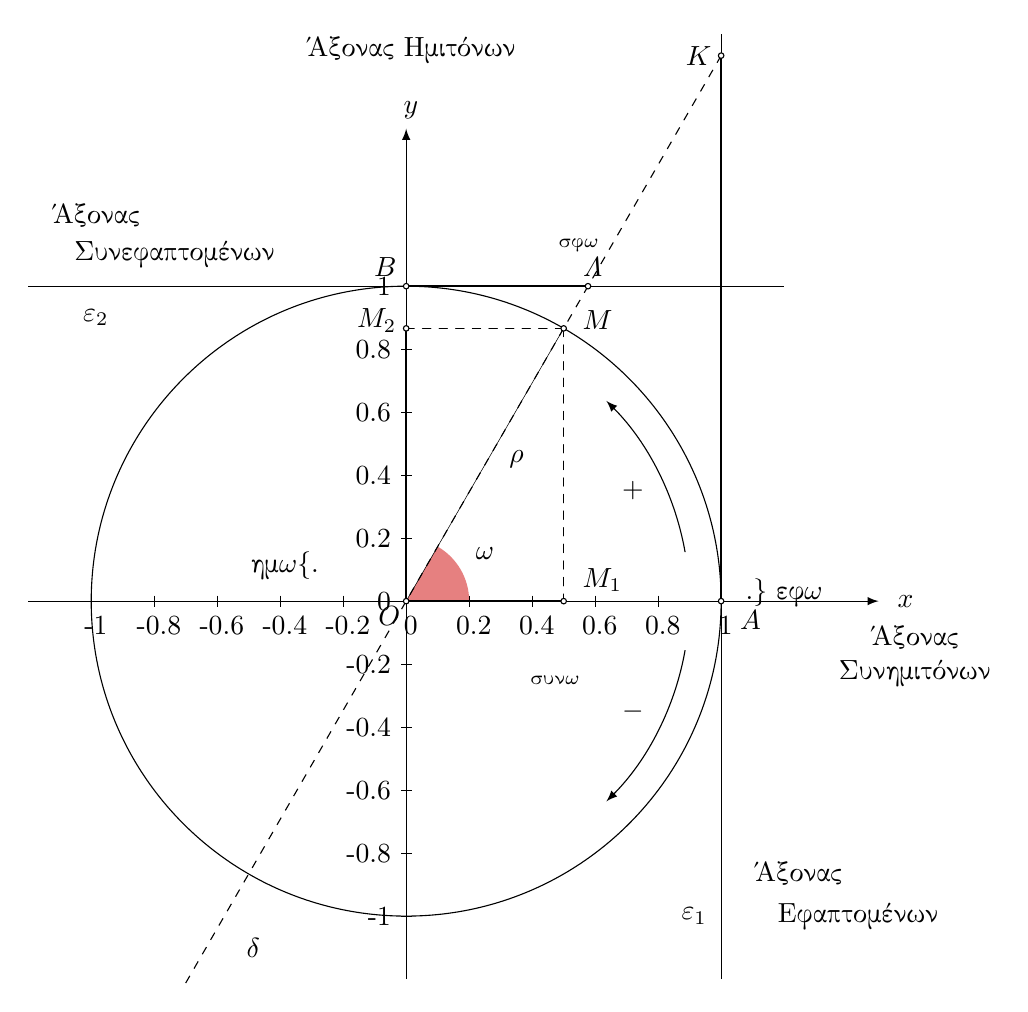
\begin{tikzpicture}[>=latex,scale=4]
\fill[fill=\xrwma!50] (0,0) -- (.2,0) arc (0:60:.2) -- cycle;
%axis
\draw[->] (-1.2,0) -- coordinate (x axis mid) (1.5,0) node[right,fill=white] {{ $ x $}};
\foreach \x in {-1,-0.8,-0.6,-0.4,-0.2,0,0.2,0.4,0.6,0.8,1}
\draw (\x,.5pt) -- (\x,-.5pt)
node[anchor=north] {{ \x}};
\foreach \y in {-1,-0.8,-0.6,-0.4,-0.2,0,0.2,0.4,0.6,0.8,1}
\draw (.5pt,\y) -- (-.5pt,\y)
node[anchor=east] {{ \y}};
\draw[->] (0,-1.2) -- (0,1.5) node[above,fill=white] {{ $ y $}};
\draw[-] (1,-1.2) -- (1,1.8);
\draw[-] (-1.2,1) -- (1.2,1);
\draw[-,thick] (0,1) -- (1.732/3,1);
\draw[-,thick] (1,0) -- (1,1.732);
\draw[-,dashed] (-.7,-1.732*0.7) -- (1,1.732);
\draw circle (1);
\coordinate (A) at (60:1);
\tkzDefPoint(0,0){O}
\tkzDefPoint(cos(pi/3),0){B}
\tkzDefPoint(0,sin(pi/3)){C}
\tkzDefPoint(1,tan(pi/3)){D}
\tkzDefPoint(cot(pi/3),1){E}
\tkzDefPoint(1,0){F}
\tkzDefPoint(0,1){G}
\tkzDrawSegment(O,A)
\tkzDrawSegments[thin,dashed](A,B A,C)
\tkzText(0,1.75){{ Άξονας Ημιτόνων}}
\tkzText(1.6,-.12){{ Άξονας}}
\tkzText(1.6,-.23){{ Συνημιτόνων}}
\tkzText(-1,1.22){{ Άξονας}}
\tkzText(-.75,1.1){{ Συνεφαπτομένων}}
\tkzText(1.23,-.87){{ Άξονας}}
\tkzText(1.42,-1){{ Εφαπτομένων}}
\tkzText(-.5,-1.1){{ $ \delta $}}
\tkzDrawSegment[thick](O,B)
\tkzDrawSegment[thick](O,C)
\tkzDrawPoints[fill=white](O,A,B,C,D,E,F,G)
\tkzText(-.4,.43){{ \textrm{ημ}$ \omega $}$\LEFTRIGHT\{.{ \rule{0pt}{28mm} } $}
\tkzText(.25,-.25){$ \undercbrace{\rule{18mm}{0mm}}_{{ \textrm{συν}\omega}} $}
\tkzText(1.2,.87){$\LEFTRIGHT.\}{ \rule{0pt}{70mm} } ${{ \textrm{εφ}$ \omega $}}}
\tkzText(.3,1.12){$ \overcbrace{\rule{20mm}{0mm}}^{{ \textrm{σφ}\omega}} $}
\tkzText(.25,.15){$ \omega $}
\tkzLabelPoint[below left,xshift=.5mm,yshift=.5mm](O){{ $ O $}}
\tkzLabelPoint[above=1mm,right](A){{ $ M $}}
\tkzLabelPoint[above right](B){{ $ M_1 $}}
\tkzLabelPoint[above=1mm, left](C){{ $ M_2 $}}
\tkzLabelPoint[left](D){{ $ K $}}
\tkzLabelPoint[above](E){{ $ \varLambda $}}
\tkzLabelPoint[below right](F){{ $ A $}}
\tkzLabelPoint[above left](G){{ $ B $}}
\draw [->] (.984*.9,.173*.9) arc (10:45:.9);
\draw [->] (.984*.9,-.173*.9) arc (-10:-45:.9);
\tkzText(.72,.35){$ + $}
\tkzText(.72,-.35){$ - $}
\tkzText(.35,.45){$ \rho $}
\tkzText(-1,.9){{ $ \varepsilon_2 $}}
\tkzText(.9,-1){{ $ \varepsilon_1 $}}
\end{tikzpicture}
\paragraph{Τριγωνομετρικοί αριθμοί βασικών γωνιών}
\begin{center}
\begin{mytblr}{} \SetCell[c=9]{c}{\textbf{\MakeUppercase{Βασικές Γωνίες}}}\\ 
\SetRow{m}\textbf{Θέση} & \SetCell{wd=1.2cm}\textbf{Σημείο άξονα} & \SetCell[c=3]{c}{\textbf{1\tss{ο} Τεταρτημόριο}} & & & \SetCell[c=4]{c}{\textbf{Σημείο άξονα}}\\
\rule[-2ex]{0pt}{5ex} \textbf{Μοίρες} & $ 0\degree $ & $ 30\degree $ & $ 45\degree $ & $ 60\degree $ & $ 90\degree $ & $ 180\degree $ & $ 270\degree $ & $ 360\degree $ \\
\textbf{Ακτίνια} & $ 0 $ & $ \frac{\pi}{6} $ & $ \frac{\pi}{4} $ & $ \frac{\pi}{3} $ & $ \frac{\pi}{2} $ & $ \pi $ & $ \frac{3\pi}{2} $ & $ 2\pi $ \\ 
\SetCell{m}\textbf{Σχήμα} & 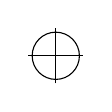
\begin{tikzpicture}
\fill[fill=red!50] (0,0) -- (.3,0) arc (0:0:.3) -- cycle;
\draw (-.35,0) -- (.35,0);
\draw (0,-.35) -- (0,.35);
\draw (0,0) circle (.3);
\coordinate (A) at (0:.3);
\draw (0,0) -- (A);
\end{tikzpicture} & 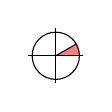
\begin{tikzpicture}
\fill[fill=red!50] (0,0) -- (.3,0) arc (0:30:.3) -- cycle;
\draw (-.35,0) -- (.35,0);
\draw (0,-.35) -- (0,.35);
\draw (0,0) circle (.3);
\coordinate (A) at (30:.3);
\draw (0,0) -- (A);
\end{tikzpicture} & 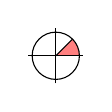
\begin{tikzpicture}
\fill[fill=red!50] (0,0) -- (.3,0) arc (0:45:.3) -- cycle;
\draw (-.35,0) -- (.35,0);
\draw (0,-.35) -- (0,.35);
\draw (0,0) circle (.3);
\coordinate (A) at (45:.3);
\draw (0,0) -- (A);
\end{tikzpicture} & 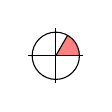
\begin{tikzpicture}
\fill[fill=red!50] (0,0) -- (.3,0) arc (0:60:.3) -- cycle;
\draw (-.35,0) -- (.35,0);
\draw (0,-.35) -- (0,.35);
\draw (0,0) circle (.3);
\coordinate (A) at (60:.3);
\draw (0,0) -- (A);
\end{tikzpicture} & 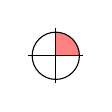
\begin{tikzpicture}
\fill[fill=red!50] (0,0) -- (.3,0) arc (0:90:.3) -- cycle;
\draw (-.35,0) -- (.35,0);
\draw (0,-.35) -- (0,.35);
\draw (0,0) circle (.3);
\coordinate (A) at (90:.3);
\draw (0,0) -- (A);
\end{tikzpicture} & 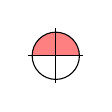
\begin{tikzpicture}
\fill[fill=red!50] (0,0) -- (.3,0) arc (0:180:.3) -- cycle;
\draw (-.35,0) -- (.35,0);
\draw (0,-.35) -- (0,.35);
\draw (0,0) circle (.3);
\end{tikzpicture} & 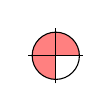
\begin{tikzpicture}
\fill[fill=red!50] (0,0) -- (.3,0) arc (0:270:.3) -- cycle;
\draw (-.35,0) -- (.35,0);
\draw (0,-.35) -- (0,.35);
\draw (0,0) circle (.3);
\end{tikzpicture} & 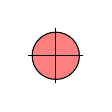
\begin{tikzpicture}
\fill[fill=red!50] (0,0) -- (.3,0) arc (0:360:.3) -- cycle;
\draw (-.35,0) -- (.35,0);
\draw (0,-.35) -- (0,.35);
\draw (0,0) circle (.3);
\end{tikzpicture} \\ 
$ \hm{\omega} $ & $ 0 $ & $ \frac{1}{2} $ & $ \frac{\sqrt{2}}{2} $ & $ \frac{\sqrt{3}}{2} $ & $ 1 $ & $ 0 $ & $ -1 $ & $ 0 $  \\ 
$ \syn{\omega} $ & $ 1 $ & $ \frac{\sqrt{3}}{2} $ & $ \frac{\sqrt{2}}{2} $ & $ \frac{1}{2} $ & $ 0 $ & $ -1 $ & $ 0 $ & $ 1 $  \\ 
$ \ef{\omega} $ & $ 0 $ & $ \frac{\sqrt{3}}{3} $ & $ 1 $ & $ \sqrt{3} $ & \begin{minipage}{.8cm}
\begin{center}
{\scriptsize Δεν\\\vspace{-1mm}ορίζεται}
\end{center}
\end{minipage} & $ 0 $ & 
\begin{minipage}{.8cm}
\begin{center}
{\scriptsize Δεν\\\vspace{-1mm}ορίζεται}
\end{center}
\end{minipage} & $ 0 $ \\
\rule[-2ex]{0pt}{4ex} $ \syf{\omega} $ & \begin{minipage}{.8cm}
\begin{center}
{\scriptsize Δεν\\\vspace{-1mm}ορίζεται}
\end{center}
\end{minipage} & $ \sqrt{3} $ & $ 1 $ & $ \frac{\sqrt{3}}{3} $ & $ 0 $ & \begin{minipage}{.8cm}
\begin{center}
{\scriptsize Δεν\\\vspace{-1mm}ορίζεται}
\end{center}
\end{minipage} & $ 0 $ & \begin{minipage}{.8cm}
\begin{center}
{\scriptsize Δεν\\\vspace{-1mm}ορίζεται}
\end{center}
\end{minipage} 
\end{mytblr}
\end{center}
\paragraph{Τριγωνομετρικές ταυτότητες}
\begin{multicols}{3}
\begin{enumerate}[itemsep=0mm]
\item $ \hm^2{\omega}+\syn^2{\omega}=1 $
\item $ \ef{\omega}={\dfrac{\hm{\omega}}{\syn{\omega}}} $
\item $ \syf{\omega}={\dfrac{\syn{\omega}}{\hm{\omega}}} $
\item $ \ef{\omega}\cdot\syf{\omega}=1 $
\item $ \syn^2{\omega}=\dfrac{1}{1+\ef^2{\omega}} $
\item $ \hm^2{\omega}=\dfrac{\ef^2{\omega}}{1+\ef^2{\omega}} $
\end{enumerate}
\end{multicols}
\paragraph{Αναγωγή στο 1ο τεταρτημόριο}
\begin{center}
\begin{mytblr}{} 
\rule[-2ex]{0pt}{5ex} \bmath{Σχέση γωνίας $ \varphi $ με την $ \omega $} & \bmath{Συμβολισμός $ \varphi= $}  & \bmath{$ \hm{\varphi} $} & \bmath{$ \syn{\varphi} $} & \bmath{$ \ef{\varphi} $} & \bmath{$ \syf{\varphi} $} \\ 
\rule[-2ex]{0pt}{5ex} Αντίθετη & $ -\omega $ & $ -\hm{\omega} $ & $ \syn{\omega} $ & $ -\ef{\omega} $ & $ -\syf{\omega} $ \\  
\rule[-2ex]{0pt}{5ex} Παραπληρωματική & $ 180\degree-\omega $ & $ \hm{\omega} $ & $ -\syn{\omega} $ & $ -\ef{\omega} $ & $ -\syf{\omega} $ \\  
Με διαφορά $180\degree$ & $ 180\degree+\omega $ & $ -\hm{\omega} $ & $ -\syn{\omega} $ & $ \ef{\omega} $ & $ \syf{\omega} $ \\  
Συμπληρωματική & $ 90\degree-\omega $ & $ \syn{\omega} $ & $ \hm{\omega} $ & $ \syf{\omega} $ & $ \ef{\omega} $ \\ 
Με διαφορά $ 90\degree $  & $ 90\degree+\omega $ & $ \syn{\omega} $ & $ -\hm{\omega} $ & $ -\syf{\omega} $ & $ -\ef{\omega} $ \\  
Με άθροισμα $ 270\degree $ & $ 270\degree-\omega $ & $ -\syn{\omega} $ & $ -\hm{\omega} $ & $ \syf{\omega} $ & $ \ef{\omega} $ \\  
Με διαφορά $ 270\degree $ & $ 270\degree+\omega $ & $ -\syn{\omega} $ & $ \hm{\omega} $ & $ -\syf{\omega} $ & $ -\ef{\omega} $ \\ 
Με άθροισμα $ 360\degree $ & $ 360\degree-\omega $ & $ -\hm{\omega} $ & $ \syn{\omega} $ & $ -\ef{\omega} $ & $ -\syf{\omega} $ \\ 
Με διαφορά $ \kappa\cdot 360\degree $ & $ \kappa\cdot360\degree+\omega $ & $ \hm{\omega} $ & $ \syn{\omega} $ & $ \ef{\omega} $ & $ \syf{\omega} $ \\  
\end{mytblr}
\end{center}
\paragraph{Τριγωνομετρικές συναρτήσεις}
Για την απλή τριγωνομετρική συνάρτηση $ f(x)=\hm{x} $ του ημιτόνου ισχύουν τα εξής :
\begin{alist}
\item Η συνάρτηση $ f $ έχει πεδίο ορισμού το σύνολο των πραγματικών αριθμών $ \mathbb{R} $.
\item Το σύνολο τιμών της $ f $ είναι το κλειστό διάστημα $ [-1,1] $.
\item Αποτελεί περιοδική συνάρτηση με περίοδο $ T=2\pi $.
\item Μελετώντας τη συνάρτηση στο διάστημα $ [0,2\pi] $ πλάτους μιας περιόδου έχουμε ότι είναι γνησίως αύξουσα στα διαστήματα $ \left[ 0,\frac{\pi}{2}\right] ,\left[ \frac{3\pi}{2},2\pi\right]  $ ενώ είναι γνησίως φθίνουσα στο διάστημα $ \left[ \frac{\pi}{2},\frac{3\pi}{2}\right]  $.
\item Παρουσιάζει μέγιστο στη θέση $ x=\frac{\pi}{2} $ την τιμή $ 1 $ και ελάχιστη τιμή $ -1 $ στη θέση $ x=\frac{3\pi}{2} $.
\end{alist}
\begin{center}
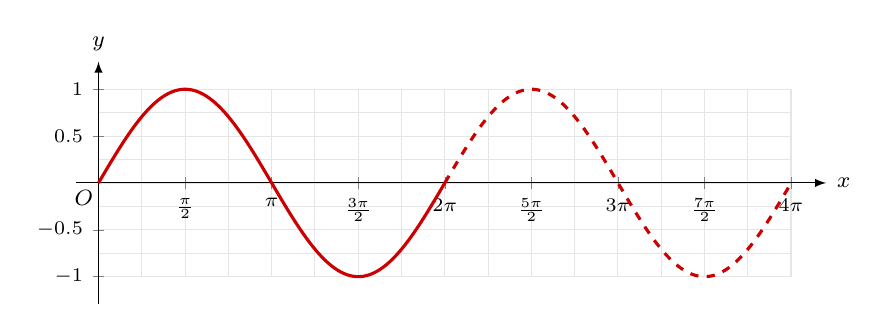
\begin{tikzpicture}
\draw[shift={(2.8mm,3.5mm)},style=help lines, xstep=0.5497cm,ystep=0.297cm,black!10] (0,0) grid (8.796,2.38);
\begin{axis}[x=.7cm,y=.7cm,xtick={
-6.28318, -4.7123889, -3.14159, -1.5708,
1.5708, 3.14159, 4.7123889, 6.28318,7.854,9.424,10.995,12.564},
xticklabels={
$-2\pi$, $-\frac{3\pi}{2}$, $-\pi$, $\frac{\pi}{2}$,
$\frac{\pi}{2}$, $\pi$, $\frac{3\pi}{2}$, $2\pi$,$\frac{5\pi}{2}$,$3\pi$,$\frac{7\pi}{2}$,$4\pi$
},ytick={-1.7,-.85,0.85,1.7},yticklabels={$-1$,$-0.5$,$0.5$,$1$},aks_on,xmin=-.4,xmax=13.2,
ymin=-2.2,ymax=2.2,xlabel={\footnotesize $ x $},
ylabel={\footnotesize $ y $},belh ar,clip=false]
\addplot[grafikh parastash,domain=0:2*pi]{1.7*sin(deg(x))};
\addplot[grafikh parastash,domain=2*pi:4*pi,dashed]{1.7*sin(deg(x))};
\end{axis}
\node at (0.0951,1.344) {\footnotesize$O$};
\end{tikzpicture}
\end{center}
\begin{alist}[resume]
\item Ως περιοδική συνάρτηση, οι τιμές, η μονοτονία τα ακρότατα και κάθε άλλο χαρακτηριστικό επαναλαμβάνονται σε κάθε διάστημα πλάτους μιας περιόδου $ 2\pi $. Τα διαστήματα αυτά θα είναι της μορφής $ [2\kappa\pi,2\left( \kappa+1\right)\pi] $ με $ \kappa\in\mathbb{Z} $.
\item Γενικά η $ f $ είναι γνησίως αύξουσα στα διαστήματα $ \left[2\kappa\pi,2\kappa\pi+\frac{\pi}{2}\right]$ και $\left[2\kappa\pi+\frac{3\pi}{2},2(\kappa+1)\pi \right]  $ ενώ είναι γνησίως φθίνουσα στα διαστήματα $ \left[2\kappa\pi+\frac{\pi}{2},\right. $  $\left. 2\kappa\pi+\frac{3\pi}{2} \right]  $ με $ \kappa\in\mathbb{Z} $.
\item Παρουσιάζει μέγιστο στις θέσεις $ x=2\kappa\pi+\frac{\pi}{2} $ την τιμή $ 1 $ και ελάχιστο στις θέσεις $ x=2\kappa\pi+\frac{3\pi}{2} $ την τιμή $ -1 $.
\item Η γραφική της παράσταση τέμνει τον οριζόντιο άξονα $ x'x $ στα σημεία με τετμημένες $ x=\kappa\pi $ με $ \kappa\in\mathbb{Z} $.
\end{alist}
\textbf{Η συνάρτηση {\boldmath$ f(x)=\syn{x} $}}\\
Για την απλή τριγωνομετρική συνάρτηση $ f(x)=\syn{x} $ του συνημιτόνου ισχύουν τα εξής :
\begin{alist}
\item Η συνάρτηση $ f $ έχει πεδίο ορισμού το σύνολο των πραγματικών αριθμών $ \mathbb{R} $.
\item Το σύνολο τιμών της $ f $ είναι το κλειστό διάστημα $ [-1,1] $.
\item Αποτελεί περιοδική συνάρτηση με περίοδο $ T=2\pi $.
\item Αν μελετήσουμε τη συνάρτηση στο διάστημα $ [0,2\pi] $ πλάτους μιας περιόδου βλέπουμε οτι είναι γνησίως αύξουσα στο διάστημα $ \left[ \pi,2\pi\right] $ ενώ είναι γνησίως φθίνουσα στο διάστημα $ \left[ 0,\pi\right]  $.
\item Παρουσιάζει μέγιστο στις θέση $ x=0 $ και $ x=2\pi $ την τιμή $ 1 $ και ελάχιστη τιμή $ -1 $ στη θέση $ x=\pi $.
\end{alist}
\begin{center}
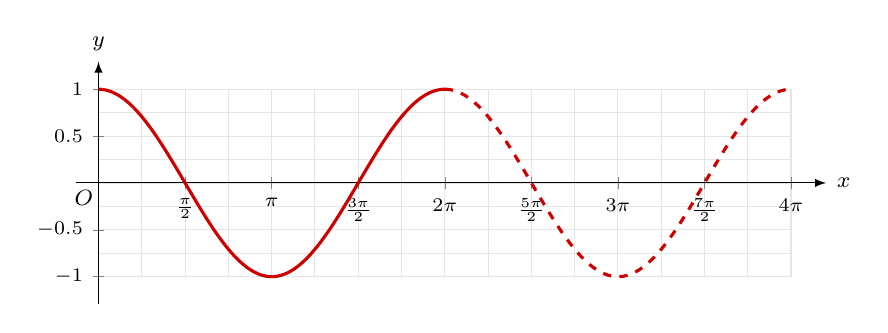
\begin{tikzpicture}
\draw[shift={(2.8mm,3.5mm)},style=help lines, xstep=0.5497cm,ystep=0.297cm,black!10] (0,0) grid (8.796,2.38);
\begin{axis}[x=.7cm,y=.7cm,xtick={
-6.28318, -4.7123889, -3.14159, -1.5708,
1.5708, 3.14159, 4.7123889, 6.28318,7.854,9.424,10.995,12.564},
xticklabels={
$-2\pi$, $-\frac{3\pi}{2}$, $-\pi$, $\frac{\pi}{2}$,
$\frac{\pi}{2}$, $\pi$, $\frac{3\pi}{2}$, $2\pi$,$\frac{5\pi}{2}$,$3\pi$,$\frac{7\pi}{2}$,$4\pi$
},ytick={-1.7,-.85,0.85,1.7},yticklabels={$-1$,$-0.5$,$0.5$,$1$},aks_on,xmin=-.4,xmax=13.2,
ymin=-2.2,ymax=2.2,xlabel={\footnotesize $ x $},
ylabel={\footnotesize $ y $},belh ar,clip=false]
\addplot[grafikh parastash,domain=0:2*pi]{1.7*cos(deg(x))};
\addplot[grafikh parastash,domain=2*pi:4*pi,dashed]{1.7*cos(deg(x))};
\end{axis}
\node at (0.0951,1.344) {\footnotesize$O$};
\end{tikzpicture}
\end{center}
\begin{alist}[resume]
\item Ως περιοδική συνάρτηση, οι ιδιότητες και τα χαρακτηριστικά επαναλαμβάνονται σε κάθε διάστημα πλάτους μιας περιόδου $ 2\pi $. Τα διαστήματα αυτά θα είναι της μορφής $ [2\kappa\pi,2\left( \kappa+1\right)\pi] $ με $ \kappa\in\mathbb{Z} $.
\item Η $ f $ είναι γνησίως αύξουσα στα διαστήματα $ \left[2\kappa\pi+\pi,2(\kappa+1)\pi\right]$ ενώ είναι γνησίως φθίνουσα στα διαστήματα $ \left[2\kappa\pi, 2\kappa\pi+\pi \right]  $ με $ \kappa\in\mathbb{Z} $.
\item Παρουσιάζει μέγιστο στις θέσεις $ x=2\kappa\pi $ και $ x=2(\kappa+1)\pi $ την τιμή $ 1 $ και ελάχιστο στις θέσεις $ x=2\kappa\pi+\pi $ την τιμή $ -1 $.
\item Η γραφική της παράσταση τέμνει τον οριζόντιο άξονα $ x'x $ στα σημεία με τετμημένες $ x=\kappa\pi+\frac{\pi}{2} $ με $ \kappa\in\mathbb{Z} $.
\end{alist}
\end{multicols}
\end{document}
